\noindent
\includegraphics[height=1.25cm]{images/pictograms/benchmark}
\includegraphics[height=1.25cm]{images/pictograms/aspect_logo}
\includegraphics[height=1.25cm]{images/pictograms/FEM}
\includegraphics[height=1.25cm]{images/pictograms/paraview}


%%%%%%%%%%%%%%%%%%%%%%%%%%%%%%%%%%%%%%%%%%%%%%%%%%%%%%%%%%%%%%%%%%%%%%%%%%%%%%%%%%%%%%%%%%%%%%%%%%%

\begin{flushright} {\tiny {\color{gray} python\_codes/fieldstone\_152/text.tex}} \end{flushright}

\lstinputlisting[language=bash,basicstyle=\small]{python_codes/fieldstone_152/keywords.key}

\par\noindent\rule{\textwidth}{0.4pt}

\begin{center}
\inpython
{\small Code: \url{https://github.com/cedrict/fieldstone/tree/master/python_codes/fieldstone_152}}
\end{center}

\par\noindent\rule{\textwidth}{0.4pt}

%{\sl This stone was developed in collaboration with Donald Duck}. \index{contributors}{D. Duck}

%\par\noindent\rule{\textwidth}{0.4pt}

%%%%%%%%%%%%%%%%%%%%%%%%%%%%%%%%%%%%%%%%%%%%%%%%%%%%%%%%%%%%%%%%%%%%%%%%%%%%%%%%%%%%%%%%%%%%%%%%%%%






























\newpage
%%%%%%%%%%%%%%%%%%%%%%%%%%%%%%%%%%%%%%%%%%%%%%%%%%
\section*{Thoughts about computing gravity inside the domain}

Following Appendix A of \textcite{thie18}, the gravity and
gravity potential of a hollow sphere of constant 
density is given by:
\[
g(r)=\frac{{\cal G}M}{r^2}
\qquad
U(r)=-\frac{{\cal G}M}{r}
\]
for $r\ge R_2$, by 
\[
g(r)=\frac{4 \pi}{3} {\cal G} \rho_0 (r-\frac{R_1^3}{r^2})
\qquad
U(r)=\frac{4\pi}{3}{\cal G} \rho_0 \left( \frac{r^2}{2}+ \frac{R_1^3}{r} \right)
-2 \pi \rho_0 {\cal G}R_2^2
\]
for $R_1\le r \le R_2$ and by 
\[
g(r)=0
\qquad
U(r)=2\pi {\cal G} \rho_0 (R_1^2-R_2^2)
\]
for $r\le R_1$.

\begin{center}
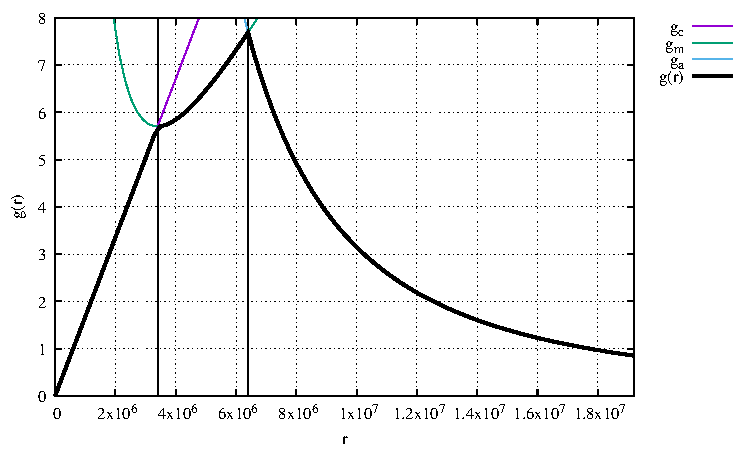
\includegraphics[width=6cm]{./python_codes/fieldstone_152/images/bench/g}
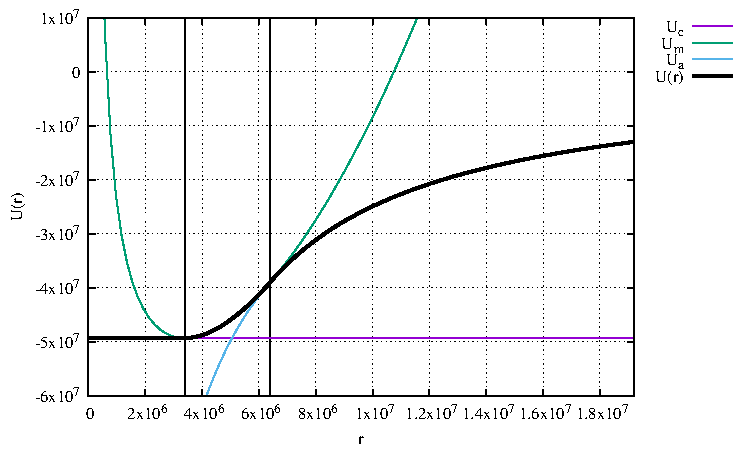
\includegraphics[width=6cm]{./python_codes/fieldstone_152/images/bench/U}\\
{\captionfont Gravity and gravity potential as a function of $r$.}
\end{center}


We start from 
\[
\Delta U = 4 \pi \rho {\cal G}
\]
or 
\[
\vec\nabla \cdot \vec\nabla  U = -\vec\nabla \cdot \vec{g} = 4 \pi \rho {\cal G}
\]
In cylindrical coordinates we would then write (axisymmetric case)
\[
\vec\nabla\cdot \vec{g} 
= \frac{1}{r} \frac{\partial }{\partial r} (r g_r) 
+\frac{\partial g_z}{\partial z}  = 4\pi \rho {\cal G}
\]
or, 
\[
\frac{g_r}{r} + \frac{\partial g_r}{\partial r} 
+\frac{\partial g_z}{\partial z}  = \hat{\rho}
\]
It would be tempting to go ahead and try to establish the 
weak form of this equations since it is $\vec{g}$ we would 
like to compute and not $U$, but it is *hopeless* as the equation 
itself is not well posed. We have 2 unknowns and only one equation!

Let us denote $\hat{\rho}=4\pi {\cal G} \rho$ and start again from 
\[
\Delta U = \hat{\rho}
\]
We could look at the expression for the Laplace operator
in cylindrical coordinates but we recognise the same type of 
PDE as the steady state heat diffusion equation, so we
will adopt the same methodology, i.e. multiplying by a test function
$W$ and integrating over the domain:
\[
\int_V W \Delta U dV = \int_V W \hat{\rho} dV
\]
However, let us think a bit more about the boundary conditions in the 
case where the solution is not known. 
On the inner boundary we have $g=0$ for a hollow sphere, 
i.e. $\vec\nabla U\cdot \vec{n}=0$, 
which we get for free by not imposing any Dirichlet bc on this boundary.
On the outer boundary, we are facing a problem: we do not know what $U$
is, so we can't prescribe it (no Dirichlet bc), and we don't know 
what its derivative is (i.e. the gravity vector) so no Neumann bc possible.
The inescapable conclusion is that *if* we would want to 
use FE to compute the gravity fields, we would need a very large domain 
($r\rightarrow \infty$) where we could prescribe $U\simeq 0$ there.













\newpage
%%%%%%%%%%%%%%%%%%%%%%%%%%%%%%%%%%%%%%%%%%%%%%%%%%%%%%%%%%%%%%%%%%%%%%%%%%%%%%%
\section*{Exp=0: Annulus convection benchmark (exp=0)}

In order to run this benchmark, the following two options must be False in the code:
\begin{lstlisting}
axisymmetric=False
surface_free_slip=False
\end{lstlisting}

This benchmark is documented in Section~\ref{MMM-ss:anconv}.

For reference, in this benchmark we solve the Stokes equation for an incompressible
isothermal fluid in an annulus of inner radius $R_1$
and outer radius $R_2$ with the following boundary conditions:
\begin{itemize}
\item Inner boundary: $\upnu_r(R_1,\theta)=0$ 
\item Outer boundary: $\upnu_r(R_2,\theta)=0$ 
\end{itemize}
and the manufactured solution takes the form:
\begin{eqnarray}
\upnu_\theta(r,\theta) &=& f(r) \cos(k\theta) \\
\upnu_r(r,\theta) &=& g(r) k  \sin(k\theta)  \\
p(r,\theta) &=& k h(r) \sin(k \theta) + \rho_0 g_r (r-R_2)  \\
\rho(r,\theta) &=& k \sin (k \theta) \aleph(r) + \rho_0 \\
\end{eqnarray}
with
\begin{eqnarray}
A &=& \frac{2(\ln R_1 - \ln R_2)} { R_2^2 \ln R_1  - R_1^2 \ln R_2}    \nn\\
B &=& \frac{R_2^2-R_1^2}{R_2^2 \ln R_1 - R_1^2 \ln R_2} \nn\\
f(r)   &=& Ar +\frac{B}{r} \nn\\
f'(r)  &=& A - \frac{B}{r^2} \nn\\
g(r)   &=& \frac{A}{2}r  +  \frac{B}{r} \ln r - \frac{1}{r} \nn\\
g'(r)  &=& \frac{A}{2}  +  \frac{B}{r^2} (1-\ln r)   + \frac{1}{r^2} \nn\\
g''(r) &=&  - \frac{B}{r^3} (3 - 2 \ln r )  \nn\\
h(r)   &=& \frac{1}{r^2}(2g-f) \nn\\
\aleph(r) &=&  -g'' - \frac{g'}{r} ( 1 - \frac{2}{r}) + \frac{g}{r^2} (k^2 + 1 -\frac{4}{r})  
- \frac{2f}{r^2}  (1-\frac{1}{r}) - \frac{f'}{r^2}   \nn
\end{eqnarray}

\begin{center}
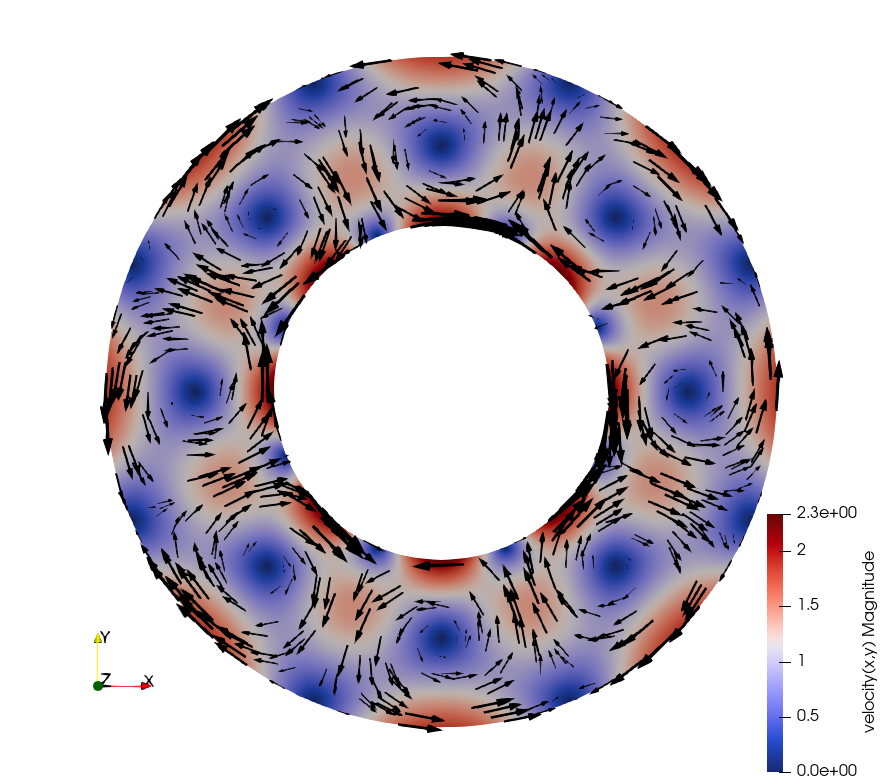
\includegraphics[width=6cm]{python_codes/fieldstone_152/images/vel}
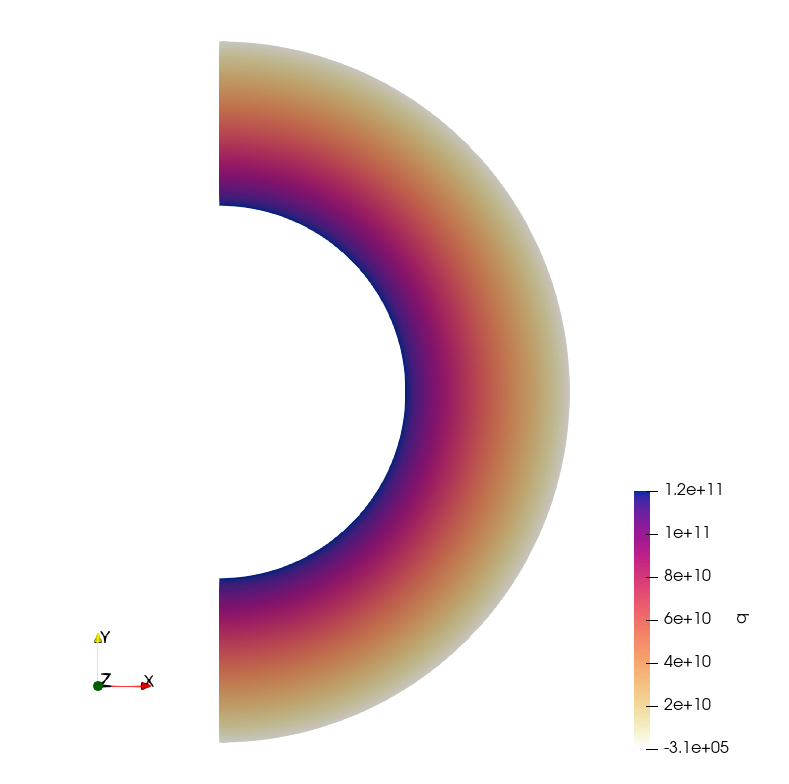
\includegraphics[width=6cm]{python_codes/fieldstone_152/images/press}\\
{\captionfont Velocity and pressure fields for $k=4$.}
\end{center}

%---------------------------------------
\subsection*{Root mean square velocity}

\begin{center}
\includegraphics[width=8.3cm]{python_codes/fieldstone_152/RESULTS/exp0/vrms}
\includegraphics[width=8.3cm]{python_codes/fieldstone_152/RESULTS/exp0/vrms_error}\\
{\captionfont Note that we define $h=(R_2-R_1)/nelr=1/nelr$.}
\end{center}

As expected linear mapping yields the worst results. However results are virtually identical for 
the three other mappings.
What is very surprising is the much higher accuracy of {\python nqperdim=2} (i.e. subparametric mapping) ?!


%---------------------------------------
\subsection*{Velocity and pressure errors}

We first look at the min/max values of the nodal velocity and pressure errors over all the nodes:
\begin{center}
\includegraphics[width=5.4cm]{python_codes/fieldstone_152/RESULTS/exp0/u_err}
\includegraphics[width=5.4cm]{python_codes/fieldstone_152/RESULTS/exp0/v_err}
\includegraphics[width=5.4cm]{python_codes/fieldstone_152/RESULTS/exp0/p_err}\\
{\captionfont min/max of $u^h(x,y)-u^{th}(x,y)$ and $v^h(x,y)-v^{th}(x,y)$, min/max of $p^h(x,y)-p^{th}(x,y)$.} 
\end{center}
We see that all measurements decrease (in amplitude) when the resolution is increased and that 
the $Q_1$ mapping yields the largest errors. 
Interestingly the subparametric case {\python nqperdim=2} seems to yield more accurate 
pressure results.

Turning now to velocity and pressure errors in the $L_2$ norm, 
as expected with the \QtwoQone element (and already shown in \stone~\ref{f21})
we recover a cubic convergence for the velocity error and quadratic for the 
pressure... almost always.

\begin{center}
\includegraphics[width=8.3cm]{python_codes/fieldstone_152/RESULTS/exp0/errv}
\includegraphics[width=8.3cm]{python_codes/fieldstone_152/RESULTS/exp0/errp}
\end{center}

Our velocity and pressure error measurements are identical to those of \aspect.
But why does the subparametric mapping yield a pressure error that is superconvergent?

%---------------------------------------
\subsection*{Strain rate errors}

Since the analytical velocity field is known so are the strain rate tensor components.
Similarly to \stone~21 this code computes the nodal strain rate components
in three different ways. 
\begin{itemize}
\item method \#1: strain rate components are computed in the middle of the element and then averaged over elements sharing a node.
\item method \#2: strain rate components are computed at each node of the element and then averaged over elements sharing a node.
\item method \#3: global recovery process as documented in Section~\ref{MMM-ss:gradrecovery}.
\end{itemize}

Errors are then computed in the same way as the velocity components.


TODO!!!!







\newpage
%%%%%%%%%%%%%%%%%%%%%%%%%%%%%%%%%%%%%%%%%%%%%%%%%%%%%%%%%%%%%%%%%%%%%%%%%%%%%%%
\section*{Exp=1: - the aquarium test (2D)}

\begin{lstlisting}
axisymmetric=False
surface_free_slip=True
\end{lstlisting}

Planet is R1=3400km, R2=6400km, g=10, rho=4000, eta=1e21.
Free slip on top, no slip at bottom. Unless specified, xi=6.
We test for resolution, mapping, nb of quadrature points.
Measuring quantities at the surface for $\theta\in[0,2\pi]$.
Obtained with {\tt script\_exp1}


\noindent
\includegraphics[width=3.5cm]{python_codes/fieldstone_152/RESULTS/exp1_2D/vel_16_m2}
\includegraphics[width=3.5cm]{python_codes/fieldstone_152/RESULTS/exp1_2D/vel_16_m3}
\includegraphics[width=3.5cm]{python_codes/fieldstone_152/RESULTS/exp1_2D/vel_16_m4}
\includegraphics[width=3.5cm]{python_codes/fieldstone_152/RESULTS/exp1_2D/vel_16_m5}
\includegraphics[width=3.5cm]{python_codes/fieldstone_152/RESULTS/exp1_2D/vel_16_m6}

\noindent
\includegraphics[width=3.5cm]{python_codes/fieldstone_152/RESULTS/exp1_2D/vel_32_m2}
\includegraphics[width=3.5cm]{python_codes/fieldstone_152/RESULTS/exp1_2D/vel_32_m3}
\includegraphics[width=3.5cm]{python_codes/fieldstone_152/RESULTS/exp1_2D/vel_32_m4}
\includegraphics[width=3.5cm]{python_codes/fieldstone_152/RESULTS/exp1_2D/vel_32_m5}
\includegraphics[width=3.5cm]{python_codes/fieldstone_152/RESULTS/exp1_2D/vel_32_m6}

\noindent
\includegraphics[width=3.5cm]{python_codes/fieldstone_152/RESULTS/exp1_2D/vel_64_m2}
\includegraphics[width=3.5cm]{python_codes/fieldstone_152/RESULTS/exp1_2D/vel_64_m3}
\includegraphics[width=3.5cm]{python_codes/fieldstone_152/RESULTS/exp1_2D/vel_64_m4}
\includegraphics[width=3.5cm]{python_codes/fieldstone_152/RESULTS/exp1_2D/vel_64_m5}
\includegraphics[width=3.5cm]{python_codes/fieldstone_152/RESULTS/exp1_2D/vel_64_m6}

\noindent
\includegraphics[width=3.5cm]{python_codes/fieldstone_152/RESULTS/exp1_2D/vel_128_m2}
\includegraphics[width=3.5cm]{python_codes/fieldstone_152/RESULTS/exp1_2D/vel_128_m3}
\includegraphics[width=3.5cm]{python_codes/fieldstone_152/RESULTS/exp1_2D/vel_128_m4}
\includegraphics[width=3.5cm]{python_codes/fieldstone_152/RESULTS/exp1_2D/vel_128_m5}
\includegraphics[width=3.5cm]{python_codes/fieldstone_152/RESULTS/exp1_2D/vel_128_m6}

\hrule

\noindent
\includegraphics[width=3.5cm]{python_codes/fieldstone_152/RESULTS/exp1_2D/qqq_16_m2}
\includegraphics[width=3.5cm]{python_codes/fieldstone_152/RESULTS/exp1_2D/qqq_16_m3}
\includegraphics[width=3.5cm]{python_codes/fieldstone_152/RESULTS/exp1_2D/qqq_16_m4}
\includegraphics[width=3.5cm]{python_codes/fieldstone_152/RESULTS/exp1_2D/qqq_16_m5}
\includegraphics[width=3.5cm]{python_codes/fieldstone_152/RESULTS/exp1_2D/qqq_16_m6}

\noindent
\includegraphics[width=3.5cm]{python_codes/fieldstone_152/RESULTS/exp1_2D/qqq_32_m2}
\includegraphics[width=3.5cm]{python_codes/fieldstone_152/RESULTS/exp1_2D/qqq_32_m3}
\includegraphics[width=3.5cm]{python_codes/fieldstone_152/RESULTS/exp1_2D/qqq_32_m4}
\includegraphics[width=3.5cm]{python_codes/fieldstone_152/RESULTS/exp1_2D/qqq_32_m5}
\includegraphics[width=3.5cm]{python_codes/fieldstone_152/RESULTS/exp1_2D/qqq_32_m6}

\noindent
\includegraphics[width=3.5cm]{python_codes/fieldstone_152/RESULTS/exp1_2D/qqq_64_m2}
\includegraphics[width=3.5cm]{python_codes/fieldstone_152/RESULTS/exp1_2D/qqq_64_m3}
\includegraphics[width=3.5cm]{python_codes/fieldstone_152/RESULTS/exp1_2D/qqq_64_m4}
\includegraphics[width=3.5cm]{python_codes/fieldstone_152/RESULTS/exp1_2D/qqq_64_m5}
\includegraphics[width=3.5cm]{python_codes/fieldstone_152/RESULTS/exp1_2D/qqq_64_m6}

\noindent
\includegraphics[width=3.5cm]{python_codes/fieldstone_152/RESULTS/exp1_2D/qqq_128_m2}
\includegraphics[width=3.5cm]{python_codes/fieldstone_152/RESULTS/exp1_2D/qqq_128_m3}
\includegraphics[width=3.5cm]{python_codes/fieldstone_152/RESULTS/exp1_2D/qqq_128_m4}
\includegraphics[width=3.5cm]{python_codes/fieldstone_152/RESULTS/exp1_2D/qqq_128_m5}
\includegraphics[width=3.5cm]{python_codes/fieldstone_152/RESULTS/exp1_2D/qqq_128_m6}

\hrule

\noindent
\includegraphics[width=3.5cm]{python_codes/fieldstone_152/RESULTS/exp1_2D/sr2_16_m2}
\includegraphics[width=3.5cm]{python_codes/fieldstone_152/RESULTS/exp1_2D/sr2_16_m3}
\includegraphics[width=3.5cm]{python_codes/fieldstone_152/RESULTS/exp1_2D/sr2_16_m4}
\includegraphics[width=3.5cm]{python_codes/fieldstone_152/RESULTS/exp1_2D/sr2_16_m5}
\includegraphics[width=3.5cm]{python_codes/fieldstone_152/RESULTS/exp1_2D/sr2_16_m6}

\noindent
\includegraphics[width=3.5cm]{python_codes/fieldstone_152/RESULTS/exp1_2D/sr2_32_m2}
\includegraphics[width=3.5cm]{python_codes/fieldstone_152/RESULTS/exp1_2D/sr2_32_m3}
\includegraphics[width=3.5cm]{python_codes/fieldstone_152/RESULTS/exp1_2D/sr2_32_m4}
\includegraphics[width=3.5cm]{python_codes/fieldstone_152/RESULTS/exp1_2D/sr2_32_m5}
\includegraphics[width=3.5cm]{python_codes/fieldstone_152/RESULTS/exp1_2D/sr2_32_m6}

\noindent
\includegraphics[width=3.5cm]{python_codes/fieldstone_152/RESULTS/exp1_2D/sr2_64_m2}
\includegraphics[width=3.5cm]{python_codes/fieldstone_152/RESULTS/exp1_2D/sr2_64_m3}
\includegraphics[width=3.5cm]{python_codes/fieldstone_152/RESULTS/exp1_2D/sr2_64_m4}
\includegraphics[width=3.5cm]{python_codes/fieldstone_152/RESULTS/exp1_2D/sr2_64_m5}
\includegraphics[width=3.5cm]{python_codes/fieldstone_152/RESULTS/exp1_2D/sr2_64_m6}

\noindent
\includegraphics[width=3.5cm]{python_codes/fieldstone_152/RESULTS/exp1_2D/sr2_128_m2}
\includegraphics[width=3.5cm]{python_codes/fieldstone_152/RESULTS/exp1_2D/sr2_128_m3}
\includegraphics[width=3.5cm]{python_codes/fieldstone_152/RESULTS/exp1_2D/sr2_128_m4}
\includegraphics[width=3.5cm]{python_codes/fieldstone_152/RESULTS/exp1_2D/sr2_128_m5}
\includegraphics[width=3.5cm]{python_codes/fieldstone_152/RESULTS/exp1_2D/sr2_128_m6}

\hrule







\newpage
%%%%%%%%%%%%%%%%%%%%%%%%%%%%%%%%%%%%%%%%%%%%%%%%%%%%%%%%%%%%%%%%%%%%%%%%%%%%%%%
\section*{Exp=1: - the aquarium test (3D)}

\begin{lstlisting}
axisymmetric=True
surface_free_slip=True
\end{lstlisting}


Planet is R1=3400km, R2=6400km, g=10, rho=4000, eta=1e21.
Free slip on all sides, no slip at bottom. Unless specified, xi=6.
We test for resolution, mapping, nb of quadrature points.
Measuring quantities at the surface for $\theta\in[0,\pi]$.
Obtained with {\tt script\_exp1}


\noindent
\includegraphics[width=3.5cm]{python_codes/fieldstone_152/RESULTS/exp1/vel_16_m2}
\includegraphics[width=3.5cm]{python_codes/fieldstone_152/RESULTS/exp1/vel_16_m3}
\includegraphics[width=3.5cm]{python_codes/fieldstone_152/RESULTS/exp1/vel_16_m4}
\includegraphics[width=3.5cm]{python_codes/fieldstone_152/RESULTS/exp1/vel_16_m5}
\includegraphics[width=3.5cm]{python_codes/fieldstone_152/RESULTS/exp1/vel_16_m6}

\noindent
\includegraphics[width=3.5cm]{python_codes/fieldstone_152/RESULTS/exp1/vel_32_m2}
\includegraphics[width=3.5cm]{python_codes/fieldstone_152/RESULTS/exp1/vel_32_m3}
\includegraphics[width=3.5cm]{python_codes/fieldstone_152/RESULTS/exp1/vel_32_m4}
\includegraphics[width=3.5cm]{python_codes/fieldstone_152/RESULTS/exp1/vel_32_m5}
\includegraphics[width=3.5cm]{python_codes/fieldstone_152/RESULTS/exp1/vel_32_m6}

\noindent
\includegraphics[width=3.5cm]{python_codes/fieldstone_152/RESULTS/exp1/vel_64_m2}
\includegraphics[width=3.5cm]{python_codes/fieldstone_152/RESULTS/exp1/vel_64_m3}
\includegraphics[width=3.5cm]{python_codes/fieldstone_152/RESULTS/exp1/vel_64_m4}
\includegraphics[width=3.5cm]{python_codes/fieldstone_152/RESULTS/exp1/vel_64_m5}
\includegraphics[width=3.5cm]{python_codes/fieldstone_152/RESULTS/exp1/vel_64_m6}

\noindent
\includegraphics[width=3.5cm]{python_codes/fieldstone_152/RESULTS/exp1/vel_128_m2}
\includegraphics[width=3.5cm]{python_codes/fieldstone_152/RESULTS/exp1/vel_128_m3}
\includegraphics[width=3.5cm]{python_codes/fieldstone_152/RESULTS/exp1/vel_128_m4}
\includegraphics[width=3.5cm]{python_codes/fieldstone_152/RESULTS/exp1/vel_128_m5}
\includegraphics[width=3.5cm]{python_codes/fieldstone_152/RESULTS/exp1/vel_128_m6}

\hrule

\noindent
\includegraphics[width=3.5cm]{python_codes/fieldstone_152/RESULTS/exp1/qqq_16_m2}
\includegraphics[width=3.5cm]{python_codes/fieldstone_152/RESULTS/exp1/qqq_16_m3}
\includegraphics[width=3.5cm]{python_codes/fieldstone_152/RESULTS/exp1/qqq_16_m4}
\includegraphics[width=3.5cm]{python_codes/fieldstone_152/RESULTS/exp1/qqq_16_m5}
\includegraphics[width=3.5cm]{python_codes/fieldstone_152/RESULTS/exp1/qqq_16_m6}

\noindent
\includegraphics[width=3.5cm]{python_codes/fieldstone_152/RESULTS/exp1/qqq_32_m2}
\includegraphics[width=3.5cm]{python_codes/fieldstone_152/RESULTS/exp1/qqq_32_m3}
\includegraphics[width=3.5cm]{python_codes/fieldstone_152/RESULTS/exp1/qqq_32_m4}
\includegraphics[width=3.5cm]{python_codes/fieldstone_152/RESULTS/exp1/qqq_32_m5}
\includegraphics[width=3.5cm]{python_codes/fieldstone_152/RESULTS/exp1/qqq_32_m6}

\noindent
\includegraphics[width=3.5cm]{python_codes/fieldstone_152/RESULTS/exp1/qqq_64_m2}
\includegraphics[width=3.5cm]{python_codes/fieldstone_152/RESULTS/exp1/qqq_64_m3}
\includegraphics[width=3.5cm]{python_codes/fieldstone_152/RESULTS/exp1/qqq_64_m4}
\includegraphics[width=3.5cm]{python_codes/fieldstone_152/RESULTS/exp1/qqq_64_m5}
\includegraphics[width=3.5cm]{python_codes/fieldstone_152/RESULTS/exp1/qqq_64_m6}

\noindent
\includegraphics[width=3.5cm]{python_codes/fieldstone_152/RESULTS/exp1/qqq_128_m2}
\includegraphics[width=3.5cm]{python_codes/fieldstone_152/RESULTS/exp1/qqq_128_m3}
\includegraphics[width=3.5cm]{python_codes/fieldstone_152/RESULTS/exp1/qqq_128_m4}
\includegraphics[width=3.5cm]{python_codes/fieldstone_152/RESULTS/exp1/qqq_128_m5}
\includegraphics[width=3.5cm]{python_codes/fieldstone_152/RESULTS/exp1/qqq_128_m6}

\hrule

\noindent
\includegraphics[width=3.5cm]{python_codes/fieldstone_152/RESULTS/exp1/sr2_16_m2}
\includegraphics[width=3.5cm]{python_codes/fieldstone_152/RESULTS/exp1/sr2_16_m3}
\includegraphics[width=3.5cm]{python_codes/fieldstone_152/RESULTS/exp1/sr2_16_m4}
\includegraphics[width=3.5cm]{python_codes/fieldstone_152/RESULTS/exp1/sr2_16_m5}
\includegraphics[width=3.5cm]{python_codes/fieldstone_152/RESULTS/exp1/sr2_16_m6}

\noindent
\includegraphics[width=3.5cm]{python_codes/fieldstone_152/RESULTS/exp1/sr2_32_m2}
\includegraphics[width=3.5cm]{python_codes/fieldstone_152/RESULTS/exp1/sr2_32_m3}
\includegraphics[width=3.5cm]{python_codes/fieldstone_152/RESULTS/exp1/sr2_32_m4}
\includegraphics[width=3.5cm]{python_codes/fieldstone_152/RESULTS/exp1/sr2_32_m5}
\includegraphics[width=3.5cm]{python_codes/fieldstone_152/RESULTS/exp1/sr2_32_m6}

\noindent
\includegraphics[width=3.5cm]{python_codes/fieldstone_152/RESULTS/exp1/sr2_64_m2}
\includegraphics[width=3.5cm]{python_codes/fieldstone_152/RESULTS/exp1/sr2_64_m3}
\includegraphics[width=3.5cm]{python_codes/fieldstone_152/RESULTS/exp1/sr2_64_m4}
\includegraphics[width=3.5cm]{python_codes/fieldstone_152/RESULTS/exp1/sr2_64_m5}
\includegraphics[width=3.5cm]{python_codes/fieldstone_152/RESULTS/exp1/sr2_64_m6}

\noindent
\includegraphics[width=3.5cm]{python_codes/fieldstone_152/RESULTS/exp1/sr2_128_m2}
\includegraphics[width=3.5cm]{python_codes/fieldstone_152/RESULTS/exp1/sr2_128_m3}
\includegraphics[width=3.5cm]{python_codes/fieldstone_152/RESULTS/exp1/sr2_128_m4}
\includegraphics[width=3.5cm]{python_codes/fieldstone_152/RESULTS/exp1/sr2_128_m5}
\includegraphics[width=3.5cm]{python_codes/fieldstone_152/RESULTS/exp1/sr2_128_m6}

\hrule

\noindent
\includegraphics[width=3.5cm]{python_codes/fieldstone_152/RESULTS/exp1/err_16_m2}
\includegraphics[width=3.5cm]{python_codes/fieldstone_152/RESULTS/exp1/err_16_m3}
\includegraphics[width=3.5cm]{python_codes/fieldstone_152/RESULTS/exp1/err_16_m4}
\includegraphics[width=3.5cm]{python_codes/fieldstone_152/RESULTS/exp1/err_16_m5}
\includegraphics[width=3.5cm]{python_codes/fieldstone_152/RESULTS/exp1/err_16_m6}

\noindent
\includegraphics[width=3.5cm]{python_codes/fieldstone_152/RESULTS/exp1/err_32_m2}
\includegraphics[width=3.5cm]{python_codes/fieldstone_152/RESULTS/exp1/err_32_m3}
\includegraphics[width=3.5cm]{python_codes/fieldstone_152/RESULTS/exp1/err_32_m4}
\includegraphics[width=3.5cm]{python_codes/fieldstone_152/RESULTS/exp1/err_32_m5}
\includegraphics[width=3.5cm]{python_codes/fieldstone_152/RESULTS/exp1/err_32_m6}

\noindent
\includegraphics[width=3.5cm]{python_codes/fieldstone_152/RESULTS/exp1/err_64_m2}
\includegraphics[width=3.5cm]{python_codes/fieldstone_152/RESULTS/exp1/err_64_m3}
\includegraphics[width=3.5cm]{python_codes/fieldstone_152/RESULTS/exp1/err_64_m4}
\includegraphics[width=3.5cm]{python_codes/fieldstone_152/RESULTS/exp1/err_64_m5}
\includegraphics[width=3.5cm]{python_codes/fieldstone_152/RESULTS/exp1/err_64_m6}

\noindent
\includegraphics[width=3.5cm]{python_codes/fieldstone_152/RESULTS/exp1/err_128_m2}
\includegraphics[width=3.5cm]{python_codes/fieldstone_152/RESULTS/exp1/err_128_m3}
\includegraphics[width=3.5cm]{python_codes/fieldstone_152/RESULTS/exp1/err_128_m4}
\includegraphics[width=3.5cm]{python_codes/fieldstone_152/RESULTS/exp1/err_128_m5}
\includegraphics[width=3.5cm]{python_codes/fieldstone_152/RESULTS/exp1/err_128_m6}

\hrule

\noindent
\includegraphics[width=3.5cm]{python_codes/fieldstone_152/RESULTS/exp1/d_t_16_m2}
\includegraphics[width=3.5cm]{python_codes/fieldstone_152/RESULTS/exp1/d_t_16_m3}
\includegraphics[width=3.5cm]{python_codes/fieldstone_152/RESULTS/exp1/d_t_16_m4}
\includegraphics[width=3.5cm]{python_codes/fieldstone_152/RESULTS/exp1/d_t_16_m5}
\includegraphics[width=3.5cm]{python_codes/fieldstone_152/RESULTS/exp1/d_t_16_m6}

\noindent
\includegraphics[width=3.5cm]{python_codes/fieldstone_152/RESULTS/exp1/d_t_32_m2}
\includegraphics[width=3.5cm]{python_codes/fieldstone_152/RESULTS/exp1/d_t_32_m3}
\includegraphics[width=3.5cm]{python_codes/fieldstone_152/RESULTS/exp1/d_t_32_m4}
\includegraphics[width=3.5cm]{python_codes/fieldstone_152/RESULTS/exp1/d_t_32_m5}
\includegraphics[width=3.5cm]{python_codes/fieldstone_152/RESULTS/exp1/d_t_32_m6}

\noindent
\includegraphics[width=3.5cm]{python_codes/fieldstone_152/RESULTS/exp1/d_t_64_m2}
\includegraphics[width=3.5cm]{python_codes/fieldstone_152/RESULTS/exp1/d_t_64_m3}
\includegraphics[width=3.5cm]{python_codes/fieldstone_152/RESULTS/exp1/d_t_64_m4}
\includegraphics[width=3.5cm]{python_codes/fieldstone_152/RESULTS/exp1/d_t_64_m5}
\includegraphics[width=3.5cm]{python_codes/fieldstone_152/RESULTS/exp1/d_t_64_m6}

\noindent
\includegraphics[width=3.5cm]{python_codes/fieldstone_152/RESULTS/exp1/d_t_128_m2}
\includegraphics[width=3.5cm]{python_codes/fieldstone_152/RESULTS/exp1/d_t_128_m3}
\includegraphics[width=3.5cm]{python_codes/fieldstone_152/RESULTS/exp1/d_t_128_m4}
\includegraphics[width=3.5cm]{python_codes/fieldstone_152/RESULTS/exp1/d_t_128_m5}
\includegraphics[width=3.5cm]{python_codes/fieldstone_152/RESULTS/exp1/d_t_128_m6}

\hrule

Conclusions:
\begin{itemize}
\item velocities are less than $10^{-6}$ cm/year 
\item pressures are within [-50,50] Pa
\item strain rates smaller than $10^{-20}$ cm/year 
\item dynamic topography is less than 1 mm at the surface 
\item it looks like nqperdim=4 is almost always the best (and cheaper than 5,6,7)
\end{itemize}


\newpage
\subsection*{Benchmark against \aspect}

Mesh is composed of 12 blocks of 16**3 elements.
Model is run on 4 cores on my laptop.

\begin{verbatim}
+---------------------------------------------+------------+------------+
| Total wallclock time elapsed since start    |       246s |            |
| Section                         | no. calls |  wall time | % of total |
+---------------------------------+-----------+------------+------------+
| Assemble Stokes system          |         1 |        37s |        15% |
| Build Stokes preconditioner     |         1 |        24s |       9.8% |
| Initialization                  |         1 |     0.218s |         0% |
| Postprocessing                  |         1 |      6.64s |       2.7% |
| Setup dof systems               |         1 |      1.47s |       0.6% |
| Setup initial conditions        |         1 |      4.11s |       1.7% |
| Setup matrices                  |         1 |        10s |       4.1% |
| Solve Stokes system             |         1 |       161s |        65% |
+---------------------------------+-----------+------------+------------+
\end{verbatim}

\begin{center}
\includegraphics[width=6.cm]{python_codes/fieldstone_152/RESULTS/exp1/aspect/mesh}
\includegraphics[width=6.cm]{python_codes/fieldstone_152/RESULTS/exp1/aspect/vel}\\
\includegraphics[width=6.cm]{python_codes/fieldstone_152/RESULTS/exp1/aspect/sr}
\includegraphics[width=6.cm]{python_codes/fieldstone_152/RESULTS/exp1/aspect/press}\\
\includegraphics[width=6.cm]{python_codes/fieldstone_152/RESULTS/exp1/aspect/dyntopo}
\end{center}

\newpage
%-------------------------------
\subsection*{Gravity benchmark}

Gravity is computed at a height of 250km above the surface. 
Results are obtained with {\tt script\_gravity\_exp1}.
Gravity is computed at 48 points for $\theta\in[0,\pi/2]$ (i.e. North pole to equator).
Resolution is nelr=16 $Q_2$ elements.

\begin{center}
\includegraphics[width=12cm]{python_codes/fieldstone_152/RESULTS/exp1/gravity/nelr32/gravity.pdf}\\
\includegraphics[width=5.6cm]{python_codes/fieldstone_152/RESULTS/exp1/gravity/nelr32/gravity_64m.pdf}
\includegraphics[width=5.6cm]{python_codes/fieldstone_152/RESULTS/exp1/gravity/nelr32/gravity_128m.pdf}
\includegraphics[width=5.6cm]{python_codes/fieldstone_152/RESULTS/exp1/gravity/nelr32/gravity_256m.pdf}\\
\includegraphics[width=8cm]{python_codes/fieldstone_152/RESULTS/exp1/gravity/nelr32/gravity_64nq.pdf}
\includegraphics[width=8cm]{python_codes/fieldstone_152/RESULTS/exp1/gravity/nelr32/gravity_128nq.pdf}
\includegraphics[width=8cm]{python_codes/fieldstone_152/RESULTS/exp1/gravity/nelr32/gravity_192nq.pdf}
\includegraphics[width=8cm]{python_codes/fieldstone_152/RESULTS/exp1/gravity/nelr32/gravity_256nq.pdf}\\
\includegraphics[width=12cm]{python_codes/fieldstone_152/RESULTS/exp1/gravity/nelr32/gravity_error.pdf}
\end{center}

Clearly the mapping does not influence results at all. The number of quadrature points does!
However the controlling factor for accuracy is the number of repetitions of the slice controlled
by {\tt nel\_phi}.

Let us now run similar experiments at higher resolution...

\begin{center}
\includegraphics[width=12cm]{python_codes/fieldstone_152/RESULTS/exp1/gravity/nelr64/gravity.pdf}\\
\includegraphics[width=5.6cm]{python_codes/fieldstone_152/RESULTS/exp1/gravity/nelr64/gravity_64m.pdf}
\includegraphics[width=5.6cm]{python_codes/fieldstone_152/RESULTS/exp1/gravity/nelr64/gravity_128m.pdf}
\includegraphics[width=5.6cm]{python_codes/fieldstone_152/RESULTS/exp1/gravity/nelr64/gravity_256m.pdf}\\
\includegraphics[width=8cm]{python_codes/fieldstone_152/RESULTS/exp1/gravity/nelr64/gravity_64nq.pdf}
\includegraphics[width=8cm]{python_codes/fieldstone_152/RESULTS/exp1/gravity/nelr64/gravity_128nq.pdf}
\includegraphics[width=8cm]{python_codes/fieldstone_152/RESULTS/exp1/gravity/nelr64/gravity_192nq.pdf}
\includegraphics[width=8cm]{python_codes/fieldstone_152/RESULTS/exp1/gravity/nelr64/gravity_256nq.pdf}\\
\includegraphics[width=12cm]{python_codes/fieldstone_152/RESULTS/exp1/gravity/nelr64/gravity_error.pdf}
\end{center}


We see that at higher resolution increasing {\tt nel\_phi} 
increases accuracy away from the pole, while 
the influence of the quadrature is now virtually inexistant.
Also, given that $g_{th}\simeq 5$, this means that the absolute error in the measurements 
are about $5\times 10^{-10}$, i.e. less than a $\mu Gal$.

\newpage
%-------------------------------
\subsection*{Gravity benchmark}

We can also use the same function to compute gravity inside the domain. 
This of course takes a lot of time since the function must be called at all
nodes. Fort this reason my implementation calls the function only on the pressure
nodes (the corners of elements). 

\begin{center}
\includegraphics[width=8cm]{python_codes/fieldstone_152/RESULTS/exp1/self_gravity/g}
\includegraphics[width=8cm]{python_codes/fieldstone_152/RESULTS/exp1/self_gravity/U}\\
{\captionfont Analytical solution.}
\end{center}

I have run the algorithm for various values of {\python nel\_phi}:

\begin{center}
\includegraphics[width=8cm]{python_codes/fieldstone_152/RESULTS/exp1/self_gravity/g_100}
\includegraphics[width=8cm]{python_codes/fieldstone_152/RESULTS/exp1/self_gravity/g_200}\\
\includegraphics[width=8cm]{python_codes/fieldstone_152/RESULTS/exp1/self_gravity/g_300}
\includegraphics[width=8cm]{python_codes/fieldstone_152/RESULTS/exp1/self_gravity/g_400}\\
\includegraphics[width=8cm]{python_codes/fieldstone_152/RESULTS/exp1/self_gravity/g_500}
\end{center}

We find that the accuracy is very low and it looks like we need *very* high values of 
{\python nel\_phi}.













%%%%%%%%%%%%%%%%%%%%%%%%%%%%%%%%%%%%%%%%%%%%%%%%%%%%%%%%%%%%%%%%%%%%%%%%%%%%%%%
\newpage
\section*{Exp=2 - blob delta rho/rho=0.1 \% (2D)}

Planet is R1=3400km, R2=6400km, g=10, rho=4000, eta=1e21.
Free slip on all sides. Unless specified, xi=6.
We test for resolution, mapping, nb of quadrature points.
Measuring quantities at the surface for $\theta\in[0,\pi]$.
single blob of density rho=3996, isoviscous with mantle.
Center of blob at y=4900km, radius is 400km.

For this experiment the code parameters are set to:
\begin{lstlisting}
exp         = 2
nelr        = 128 
visu        = 1
nqperdim    = 3
mapping     = 'Q2' 
xi          = 6
etablobstar = 1
rhoblobstar = 0.999
yblob       = 4900e3
Rblob       = 400e3
etalithstar = 1
\end{lstlisting}

The input file for \aspect{} is in {\tt RESULTS/exp2\_2D/aspect/}.


\begin{center}
\includegraphics[width=5.6cm]{python_codes/fieldstone_152/RESULTS/exp2_2D/rho}
\includegraphics[width=5.6cm]{python_codes/fieldstone_152/RESULTS/exp2_2D/mesh}
\includegraphics[width=5.6cm]{python_codes/fieldstone_152/RESULTS/exp2_2D/vel}\\
\includegraphics[width=12cm]{python_codes/fieldstone_152/RESULTS/exp2_2D/aspect/dynamic_topography.pdf}\\
{\captionfont Dynamic topography obtain with this \stone against the one obtained with \aspect.}
\end{center}



%%%%%%%%%%%%%%%%%%%%%%%%%%%%%%%%%%%%%%%%%%%%%%%%%%%%%%%%%%%%%%%%%%%%%%%%%%%%%%%
\newpage
\section*{Exp=2 - blob delta rho/rho=0.1 \% (3D)}

Planet is R1=3400km, R2=6400km, g=10, rho=4000, eta=1e21.
Free slip on all sides. Unless specified, xi=6.
We test for resolution, mapping, nb of quadrature points.
Measuring quantities at the surface for $\theta\in[0,\pi]$.
single blob of density rho=3996, isoviscous with mantle.
Center of blob at y=4900km, radius is 400km.
Obtained with {\tt script\_exp2}.

\noindent
\includegraphics[width=3.5cm]{python_codes/fieldstone_152/RESULTS/exp2/vel_16_m2}
\includegraphics[width=3.5cm]{python_codes/fieldstone_152/RESULTS/exp2/vel_16_m3}
\includegraphics[width=3.5cm]{python_codes/fieldstone_152/RESULTS/exp2/vel_16_m4}
\includegraphics[width=3.5cm]{python_codes/fieldstone_152/RESULTS/exp2/vel_16_m5}
\includegraphics[width=3.5cm]{python_codes/fieldstone_152/RESULTS/exp2/vel_16_m6}

\noindent
\includegraphics[width=3.5cm]{python_codes/fieldstone_152/RESULTS/exp2/vel_32_m2}
\includegraphics[width=3.5cm]{python_codes/fieldstone_152/RESULTS/exp2/vel_32_m3}
\includegraphics[width=3.5cm]{python_codes/fieldstone_152/RESULTS/exp2/vel_32_m4}
\includegraphics[width=3.5cm]{python_codes/fieldstone_152/RESULTS/exp2/vel_32_m5}
\includegraphics[width=3.5cm]{python_codes/fieldstone_152/RESULTS/exp2/vel_32_m6}

\noindent
\includegraphics[width=3.5cm]{python_codes/fieldstone_152/RESULTS/exp2/vel_64_m2}
\includegraphics[width=3.5cm]{python_codes/fieldstone_152/RESULTS/exp2/vel_64_m3}
\includegraphics[width=3.5cm]{python_codes/fieldstone_152/RESULTS/exp2/vel_64_m4}
\includegraphics[width=3.5cm]{python_codes/fieldstone_152/RESULTS/exp2/vel_64_m5}
\includegraphics[width=3.5cm]{python_codes/fieldstone_152/RESULTS/exp2/vel_64_m6}

\hrule

\noindent
\includegraphics[width=3.5cm]{python_codes/fieldstone_152/RESULTS/exp2/qqq_16_m2}
\includegraphics[width=3.5cm]{python_codes/fieldstone_152/RESULTS/exp2/qqq_16_m3}
\includegraphics[width=3.5cm]{python_codes/fieldstone_152/RESULTS/exp2/qqq_16_m4}
\includegraphics[width=3.5cm]{python_codes/fieldstone_152/RESULTS/exp2/qqq_16_m5}
\includegraphics[width=3.5cm]{python_codes/fieldstone_152/RESULTS/exp2/qqq_16_m6}

\noindent
\includegraphics[width=3.5cm]{python_codes/fieldstone_152/RESULTS/exp2/qqq_32_m2}
\includegraphics[width=3.5cm]{python_codes/fieldstone_152/RESULTS/exp2/qqq_32_m3}
\includegraphics[width=3.5cm]{python_codes/fieldstone_152/RESULTS/exp2/qqq_32_m4}
\includegraphics[width=3.5cm]{python_codes/fieldstone_152/RESULTS/exp2/qqq_32_m5}
\includegraphics[width=3.5cm]{python_codes/fieldstone_152/RESULTS/exp2/qqq_32_m6}

\noindent
\includegraphics[width=3.5cm]{python_codes/fieldstone_152/RESULTS/exp2/qqq_64_m2}
\includegraphics[width=3.5cm]{python_codes/fieldstone_152/RESULTS/exp2/qqq_64_m3}
\includegraphics[width=3.5cm]{python_codes/fieldstone_152/RESULTS/exp2/qqq_64_m4}
\includegraphics[width=3.5cm]{python_codes/fieldstone_152/RESULTS/exp2/qqq_64_m5}
\includegraphics[width=3.5cm]{python_codes/fieldstone_152/RESULTS/exp2/qqq_64_m6}

\hrule

\noindent
\includegraphics[width=3.5cm]{python_codes/fieldstone_152/RESULTS/exp2/sr2_16_m2}
\includegraphics[width=3.5cm]{python_codes/fieldstone_152/RESULTS/exp2/sr2_16_m3}
\includegraphics[width=3.5cm]{python_codes/fieldstone_152/RESULTS/exp2/sr2_16_m4}
\includegraphics[width=3.5cm]{python_codes/fieldstone_152/RESULTS/exp2/sr2_16_m5}
\includegraphics[width=3.5cm]{python_codes/fieldstone_152/RESULTS/exp2/sr2_16_m6}

\noindent
\includegraphics[width=3.5cm]{python_codes/fieldstone_152/RESULTS/exp2/sr2_32_m2}
\includegraphics[width=3.5cm]{python_codes/fieldstone_152/RESULTS/exp2/sr2_32_m3}
\includegraphics[width=3.5cm]{python_codes/fieldstone_152/RESULTS/exp2/sr2_32_m4}
\includegraphics[width=3.5cm]{python_codes/fieldstone_152/RESULTS/exp2/sr2_32_m5}
\includegraphics[width=3.5cm]{python_codes/fieldstone_152/RESULTS/exp2/sr2_32_m6}

\noindent
\includegraphics[width=3.5cm]{python_codes/fieldstone_152/RESULTS/exp2/sr2_64_m2}
\includegraphics[width=3.5cm]{python_codes/fieldstone_152/RESULTS/exp2/sr2_64_m3}
\includegraphics[width=3.5cm]{python_codes/fieldstone_152/RESULTS/exp2/sr2_64_m4}
\includegraphics[width=3.5cm]{python_codes/fieldstone_152/RESULTS/exp2/sr2_64_m5}
\includegraphics[width=3.5cm]{python_codes/fieldstone_152/RESULTS/exp2/sr2_64_m6}

\hrule

\noindent
\includegraphics[width=3.5cm]{python_codes/fieldstone_152/RESULTS/exp2/err_16_m2}
\includegraphics[width=3.5cm]{python_codes/fieldstone_152/RESULTS/exp2/err_16_m3}
\includegraphics[width=3.5cm]{python_codes/fieldstone_152/RESULTS/exp2/err_16_m4}
\includegraphics[width=3.5cm]{python_codes/fieldstone_152/RESULTS/exp2/err_16_m5}
\includegraphics[width=3.5cm]{python_codes/fieldstone_152/RESULTS/exp2/err_16_m6}

\noindent
\includegraphics[width=3.5cm]{python_codes/fieldstone_152/RESULTS/exp2/err_32_m2}
\includegraphics[width=3.5cm]{python_codes/fieldstone_152/RESULTS/exp2/err_32_m3}
\includegraphics[width=3.5cm]{python_codes/fieldstone_152/RESULTS/exp2/err_32_m4}
\includegraphics[width=3.5cm]{python_codes/fieldstone_152/RESULTS/exp2/err_32_m5}
\includegraphics[width=3.5cm]{python_codes/fieldstone_152/RESULTS/exp2/err_32_m6}

\noindent
\includegraphics[width=3.5cm]{python_codes/fieldstone_152/RESULTS/exp2/err_64_m2}
\includegraphics[width=3.5cm]{python_codes/fieldstone_152/RESULTS/exp2/err_64_m3}
\includegraphics[width=3.5cm]{python_codes/fieldstone_152/RESULTS/exp2/err_64_m4}
\includegraphics[width=3.5cm]{python_codes/fieldstone_152/RESULTS/exp2/err_64_m5}
\includegraphics[width=3.5cm]{python_codes/fieldstone_152/RESULTS/exp2/err_64_m6}

\hrule

\noindent
\includegraphics[width=3.5cm]{python_codes/fieldstone_152/RESULTS/exp2/d_t_16_m2}
\includegraphics[width=3.5cm]{python_codes/fieldstone_152/RESULTS/exp2/d_t_16_m3}
\includegraphics[width=3.5cm]{python_codes/fieldstone_152/RESULTS/exp2/d_t_16_m4}
\includegraphics[width=3.5cm]{python_codes/fieldstone_152/RESULTS/exp2/d_t_16_m5}
\includegraphics[width=3.5cm]{python_codes/fieldstone_152/RESULTS/exp2/d_t_16_m6}

\noindent
\includegraphics[width=3.5cm]{python_codes/fieldstone_152/RESULTS/exp2/d_t_32_m2}
\includegraphics[width=3.5cm]{python_codes/fieldstone_152/RESULTS/exp2/d_t_32_m3}
\includegraphics[width=3.5cm]{python_codes/fieldstone_152/RESULTS/exp2/d_t_32_m4}
\includegraphics[width=3.5cm]{python_codes/fieldstone_152/RESULTS/exp2/d_t_32_m5}
\includegraphics[width=3.5cm]{python_codes/fieldstone_152/RESULTS/exp2/d_t_32_m6}

\noindent
\includegraphics[width=3.5cm]{python_codes/fieldstone_152/RESULTS/exp2/d_t_64_m2}
\includegraphics[width=3.5cm]{python_codes/fieldstone_152/RESULTS/exp2/d_t_64_m3}
\includegraphics[width=3.5cm]{python_codes/fieldstone_152/RESULTS/exp2/d_t_64_m4}
\includegraphics[width=3.5cm]{python_codes/fieldstone_152/RESULTS/exp2/d_t_64_m5}
\includegraphics[width=3.5cm]{python_codes/fieldstone_152/RESULTS/exp2/d_t_64_m6}

\hrule

\includegraphics[width=3.5cm]{python_codes/fieldstone_152/RESULTS/exp2/vel_64_xi}


Conclusions:
\begin{itemize}
\item no need to run nelr=64 models.
\item at sufficient resolution, xi, nqperdim and mapping do not matter 
much 
\item main controlling factor is resolution (nelr)
\end{itemize}


\begin{center}
\includegraphics[width=5.6cm]{python_codes/fieldstone_152/RESULTS/exp2/rho}
\includegraphics[width=5.6cm]{python_codes/fieldstone_152/RESULTS/exp2/vel}
\includegraphics[width=5.6cm]{python_codes/fieldstone_152/RESULTS/exp2/vel2}\\
\includegraphics[width=5.6cm]{python_codes/fieldstone_152/RESULTS/exp2/sr2}
\includegraphics[width=5.6cm]{python_codes/fieldstone_152/RESULTS/exp2/press}
\end{center}



\begin{center}
\includegraphics[width=5.6cm]{python_codes/fieldstone_152/RESULTS/exp2/aspect/mesh}
\includegraphics[width=5.6cm]{python_codes/fieldstone_152/RESULTS/exp2/aspect/vel}
\includegraphics[width=5.6cm]{python_codes/fieldstone_152/RESULTS/exp2/aspect/press}\\
\includegraphics[width=12cm]{python_codes/fieldstone_152/RESULTS/exp2/aspect/dynamic_topography.pdf}\\
\end{center}



\newpage
%-------------------------------
\subsection*{Gravity benchmark}

Gravity is computed at a height of 250km above the surface. 
Note that we have here modified the {\python density.py} function so 
that the mantle has zero density and the blob 400. 
Results are obtained with {\tt script\_gravity\_exp2}.
All other parameters are identical to previous experiments.

\begin{center}
\includegraphics[width=6cm]{python_codes/fieldstone_152/RESULTS/exp2/gravity/gravity.png}
\includegraphics[width=9cm]{python_codes/fieldstone_152/RESULTS/exp2/gravity/fourslices.png}
\end{center}

The issue here is that the density is elemental. At medium resolution, the blob is not 
very well discretised so that its actual mass is not equal to its analytical value. 
We set the resolution to {\python nelr=32}.

\begin{center}
\includegraphics[width=8cm]{python_codes/fieldstone_152/RESULTS/exp2/gravity/nelr32/gravity.pdf}
\includegraphics[width=8cm]{python_codes/fieldstone_152/RESULTS/exp2/gravity/nelr32/gravity_error.pdf}
\end{center}

Setting now {\python nelr=64,96,128} (from left to right):

\begin{center}
\includegraphics[width=5.6cm]{python_codes/fieldstone_152/RESULTS/exp2/gravity/nelr64/gravity.pdf}
\includegraphics[width=5.6cm]{python_codes/fieldstone_152/RESULTS/exp2/gravity/nelr96/gravity.pdf}
\includegraphics[width=5.6cm]{python_codes/fieldstone_152/RESULTS/exp2/gravity/nelr128/gravity.pdf}\\
\includegraphics[width=5.6cm]{python_codes/fieldstone_152/RESULTS/exp2/gravity/nelr64/gravity_error.pdf}
\includegraphics[width=5.6cm]{python_codes/fieldstone_152/RESULTS/exp2/gravity/nelr96/gravity_error.pdf}
\includegraphics[width=5.6cm]{python_codes/fieldstone_152/RESULTS/exp2/gravity/nelr128/gravity_error.pdf}\\
\end{center}

Conclusion: The benchmark is succesfull. 
The accuracy will be first and foremost controlled by how well the blob can be discretised, 
i.e. the resolution of the mesh. 





%%%%%%%%%%%%%%%%%%%%%%%%%%%%%%%%%%%%%%%%%%%%%%%%%%%%%%%%%%%%%%%%%%%%%%%%%%%%%%%
\newpage
\section{Exp3 - delta rho/rho=0.1 \%}

Planet is R1=3400km, R2=6400km, g=10, rho=4000, eta=1e21.
Free slip on all sides. Unless specified, xi=6.
We test for resolution, mapping, nb of quadrature points.
Measuring quantities at the surface for $\theta\in[0,\pi]$.
nqperdim $>$5  not needed. 

\begin{lstlisting}
r=np.sqrt(x*x+y*y)
theta=np.pi/2-np.arctan2(y,x)
if theta<np.pi/8 and r>R1+3*(R2-R1)/8 and r<R1+5*(R2-R1)/8:
   val*=rhoblobstar
\end{lstlisting}

Single spherical cap of density rho=3996, isoviscous with mantle,
designed in such a way that there are no elements cut by the edges of it.

Results obtained with {\tt script\_exp3}.

\begin{center}
\includegraphics[width=5.6cm]{python_codes/fieldstone_152/RESULTS/exp3/rho}
\includegraphics[width=5.6cm]{python_codes/fieldstone_152/RESULTS/exp3/vel}
\includegraphics[width=5.6cm]{python_codes/fieldstone_152/RESULTS/exp3/press}
\end{center}

\noindent
\includegraphics[width=3.5cm]{python_codes/fieldstone_152/RESULTS/exp3/vel_16_m2}
\includegraphics[width=3.5cm]{python_codes/fieldstone_152/RESULTS/exp3/vel_16_m3}
\includegraphics[width=3.5cm]{python_codes/fieldstone_152/RESULTS/exp3/vel_16_m4}
\includegraphics[width=3.5cm]{python_codes/fieldstone_152/RESULTS/exp3/vel_16_m5}
\includegraphics[width=3.5cm]{python_codes/fieldstone_152/RESULTS/exp3/vel_16_m6}

\noindent
\includegraphics[width=3.5cm]{python_codes/fieldstone_152/RESULTS/exp3/vel_32_m2}
\includegraphics[width=3.5cm]{python_codes/fieldstone_152/RESULTS/exp3/vel_32_m3}
\includegraphics[width=3.5cm]{python_codes/fieldstone_152/RESULTS/exp3/vel_32_m4}
\includegraphics[width=3.5cm]{python_codes/fieldstone_152/RESULTS/exp3/vel_32_m5}
\includegraphics[width=3.5cm]{python_codes/fieldstone_152/RESULTS/exp3/vel_32_m6}

\noindent
\includegraphics[width=3.5cm]{python_codes/fieldstone_152/RESULTS/exp3/vel_64_m2}
\includegraphics[width=3.5cm]{python_codes/fieldstone_152/RESULTS/exp3/vel_64_m3}
\includegraphics[width=3.5cm]{python_codes/fieldstone_152/RESULTS/exp3/vel_64_m4}
\includegraphics[width=3.5cm]{python_codes/fieldstone_152/RESULTS/exp3/vel_64_m5}
\includegraphics[width=3.5cm]{python_codes/fieldstone_152/RESULTS/exp3/vel_64_m6}

\hrule

\noindent
\includegraphics[width=3.5cm]{python_codes/fieldstone_152/RESULTS/exp3/qqq_16_m2}
\includegraphics[width=3.5cm]{python_codes/fieldstone_152/RESULTS/exp3/qqq_16_m3}
\includegraphics[width=3.5cm]{python_codes/fieldstone_152/RESULTS/exp3/qqq_16_m4}
\includegraphics[width=3.5cm]{python_codes/fieldstone_152/RESULTS/exp3/qqq_16_m5}
\includegraphics[width=3.5cm]{python_codes/fieldstone_152/RESULTS/exp3/qqq_16_m6}

\noindent
\includegraphics[width=3.5cm]{python_codes/fieldstone_152/RESULTS/exp3/qqq_32_m2}
\includegraphics[width=3.5cm]{python_codes/fieldstone_152/RESULTS/exp3/qqq_32_m3}
\includegraphics[width=3.5cm]{python_codes/fieldstone_152/RESULTS/exp3/qqq_32_m4}
\includegraphics[width=3.5cm]{python_codes/fieldstone_152/RESULTS/exp3/qqq_32_m5}
\includegraphics[width=3.5cm]{python_codes/fieldstone_152/RESULTS/exp3/qqq_32_m6}

\noindent
\includegraphics[width=3.5cm]{python_codes/fieldstone_152/RESULTS/exp3/qqq_64_m2}
\includegraphics[width=3.5cm]{python_codes/fieldstone_152/RESULTS/exp3/qqq_64_m3}
\includegraphics[width=3.5cm]{python_codes/fieldstone_152/RESULTS/exp3/qqq_64_m4}
\includegraphics[width=3.5cm]{python_codes/fieldstone_152/RESULTS/exp3/qqq_64_m5}
\includegraphics[width=3.5cm]{python_codes/fieldstone_152/RESULTS/exp3/qqq_64_m6}

\hrule

\noindent
\includegraphics[width=3.5cm]{python_codes/fieldstone_152/RESULTS/exp3/sr2_16_m2}
\includegraphics[width=3.5cm]{python_codes/fieldstone_152/RESULTS/exp3/sr2_16_m3}
\includegraphics[width=3.5cm]{python_codes/fieldstone_152/RESULTS/exp3/sr2_16_m4}
\includegraphics[width=3.5cm]{python_codes/fieldstone_152/RESULTS/exp3/sr2_16_m5}
\includegraphics[width=3.5cm]{python_codes/fieldstone_152/RESULTS/exp3/sr2_16_m6}

\noindent
\includegraphics[width=3.5cm]{python_codes/fieldstone_152/RESULTS/exp3/sr2_32_m2}
\includegraphics[width=3.5cm]{python_codes/fieldstone_152/RESULTS/exp3/sr2_32_m3}
\includegraphics[width=3.5cm]{python_codes/fieldstone_152/RESULTS/exp3/sr2_32_m4}
\includegraphics[width=3.5cm]{python_codes/fieldstone_152/RESULTS/exp3/sr2_32_m5}
\includegraphics[width=3.5cm]{python_codes/fieldstone_152/RESULTS/exp3/sr2_32_m6}

\noindent
\includegraphics[width=3.5cm]{python_codes/fieldstone_152/RESULTS/exp3/sr2_64_m2}
\includegraphics[width=3.5cm]{python_codes/fieldstone_152/RESULTS/exp3/sr2_64_m3}
\includegraphics[width=3.5cm]{python_codes/fieldstone_152/RESULTS/exp3/sr2_64_m4}
\includegraphics[width=3.5cm]{python_codes/fieldstone_152/RESULTS/exp3/sr2_64_m5}
\includegraphics[width=3.5cm]{python_codes/fieldstone_152/RESULTS/exp3/sr2_64_m6}

\hrule

\noindent
\includegraphics[width=3.5cm]{python_codes/fieldstone_152/RESULTS/exp3/err_16_m2}
\includegraphics[width=3.5cm]{python_codes/fieldstone_152/RESULTS/exp3/err_16_m3}
\includegraphics[width=3.5cm]{python_codes/fieldstone_152/RESULTS/exp3/err_16_m4}
\includegraphics[width=3.5cm]{python_codes/fieldstone_152/RESULTS/exp3/err_16_m5}
\includegraphics[width=3.5cm]{python_codes/fieldstone_152/RESULTS/exp3/err_16_m6}

\noindent
\includegraphics[width=3.5cm]{python_codes/fieldstone_152/RESULTS/exp3/err_32_m2}
\includegraphics[width=3.5cm]{python_codes/fieldstone_152/RESULTS/exp3/err_32_m3}
\includegraphics[width=3.5cm]{python_codes/fieldstone_152/RESULTS/exp3/err_32_m4}
\includegraphics[width=3.5cm]{python_codes/fieldstone_152/RESULTS/exp3/err_32_m5}
\includegraphics[width=3.5cm]{python_codes/fieldstone_152/RESULTS/exp3/err_32_m6}

\noindent
\includegraphics[width=3.5cm]{python_codes/fieldstone_152/RESULTS/exp3/err_64_m2}
\includegraphics[width=3.5cm]{python_codes/fieldstone_152/RESULTS/exp3/err_64_m3}
\includegraphics[width=3.5cm]{python_codes/fieldstone_152/RESULTS/exp3/err_64_m4}
\includegraphics[width=3.5cm]{python_codes/fieldstone_152/RESULTS/exp3/err_64_m5}
\includegraphics[width=3.5cm]{python_codes/fieldstone_152/RESULTS/exp3/err_64_m6}

\hrule

\noindent
\includegraphics[width=3.5cm]{python_codes/fieldstone_152/RESULTS/exp3/d_t_16_m2}
\includegraphics[width=3.5cm]{python_codes/fieldstone_152/RESULTS/exp3/d_t_16_m3}
\includegraphics[width=3.5cm]{python_codes/fieldstone_152/RESULTS/exp3/d_t_16_m4}
\includegraphics[width=3.5cm]{python_codes/fieldstone_152/RESULTS/exp3/d_t_16_m5}
\includegraphics[width=3.5cm]{python_codes/fieldstone_152/RESULTS/exp3/d_t_16_m6}

\noindent
\includegraphics[width=3.5cm]{python_codes/fieldstone_152/RESULTS/exp3/d_t_32_m2}
\includegraphics[width=3.5cm]{python_codes/fieldstone_152/RESULTS/exp3/d_t_32_m3}
\includegraphics[width=3.5cm]{python_codes/fieldstone_152/RESULTS/exp3/d_t_32_m4}
\includegraphics[width=3.5cm]{python_codes/fieldstone_152/RESULTS/exp3/d_t_32_m5}
\includegraphics[width=3.5cm]{python_codes/fieldstone_152/RESULTS/exp3/d_t_32_m6}

\noindent
\includegraphics[width=3.5cm]{python_codes/fieldstone_152/RESULTS/exp3/d_t_64_m2}
\includegraphics[width=3.5cm]{python_codes/fieldstone_152/RESULTS/exp3/d_t_64_m3}
\includegraphics[width=3.5cm]{python_codes/fieldstone_152/RESULTS/exp3/d_t_64_m4}
\includegraphics[width=3.5cm]{python_codes/fieldstone_152/RESULTS/exp3/d_t_64_m5}
\includegraphics[width=3.5cm]{python_codes/fieldstone_152/RESULTS/exp3/d_t_64_m6}

\hrule

\includegraphics[width=3.5cm]{python_codes/fieldstone_152/RESULTS/exp3/vel_32_xi}
\includegraphics[width=3.5cm]{python_codes/fieldstone_152/RESULTS/exp3/vel_64_xi}

Conclusions:
\begin{itemize}
\item higher quadrature has no effect
\item at sufficient resolution, xi, nqperdim and mapping do not matter much 
\item main controlling factor is resolution (nelr)
\end{itemize}









\newpage
%%%%%%%%%%%%%%%%%%%%%%%%%%%%%%%%%%%%%%%%%%%%%%%%%%%%%%%%%%%%%%%%%%%%%%%%%%%%%%%%%%%%%%%%%%%%%%%%%%%
\par\noindent\rule{\textwidth}{0.4pt}

%\vspace{.5cm}
%\begin{center}
%\fbox{\begin{minipage}{0.9\textwidth}
%{\color{teal}To Do, open questions, future work?}
%\begin{itemize}
%\item do smthg
%\end{itemize}
%\end{minipage}}
%\end{center}

%%%%%%%%%%%%%%%%%%%%%%%%%%%%%%%%%%%%%%%%%%%%%%%%%%%%%%%%%%%%%%%%%%%%%%%%%%%%%%%%%%%%%%%%%%%%%%%%%%%
\vspace{.5cm}

\noindent\Literature:\\
\fullcite{zizh92a}\\
\fullcite{zizh92b}

should i do a systematic study of normal for mid edge node of elements near corners?

should i implement CBF too ?

try free surface?!
